\documentclass{article}
\usepackage{tikz}
\begin{document}
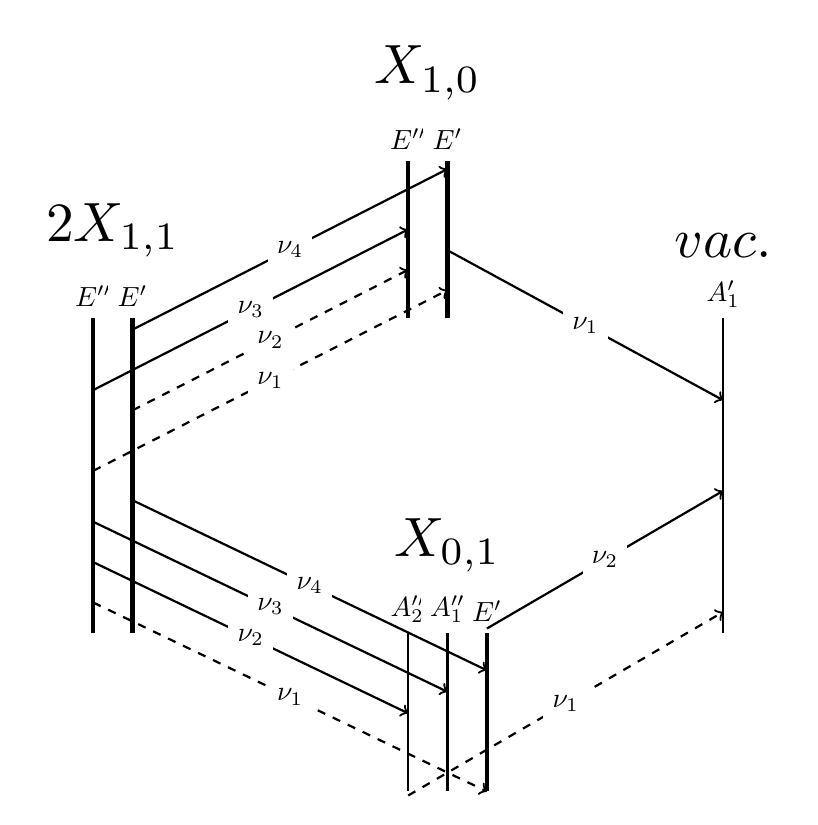
\begin{tikzpicture}[scale=1]
\draw[ultra thick] (0,1) -- (0,5) node[above=0pt,fill=white,pos=1.0] {$E''$};
\draw[ultra thick] (0.5,1) -- (0.5,5) node[above=0pt,fill=white,pos=1.0] {$E'$};
\path (0,5) -- (0.5,5) node[above=15pt,fill=white,pos=0.5,scale=2] {$2X_{1,1}$};
\draw[thick] (4,-1) -- (4,1) node[above=0pt,fill=white,pos=1.0] {$A_2''$};
\draw[thick] (4.5,-1) -- (4.5,1) node[above=0pt,fill=white,pos=1.0] {$A_1''$};
\draw[ultra thick] (5,-1) -- (5,1) node[above=0pt,fill=white,pos=1.0] {$E'$};
\path (4,1) -- (5,1) node[above=15pt,fill=white,pos=0.5,scale=2] {$X_{0,1}$};
\draw[ultra thick] (4,5) -- (4,7) node[above=0pt,fill=white,pos=1.0] {$E''$};
\draw[ultra thick] (4.5,5) -- (4.5,7) node[above=0pt,fill=white,pos=1.0] {$E'$};
\path (4,7) -- (4.5,7) node[above=15pt,fill=white,pos=0.5,scale=2] {$X_{1,0}$};
\draw[thick] (8,1) -- (8,5) node[above=0pt,fill=white,pos=1.0] {$A_1'$};
\path (8,5) -- (8,5) node[above=15pt,fill=white,pos=0.5,scale=2] {$vac.$};
\draw[dashed,->,thick] (0,1.39077) -- (5,-1.00923) node[fill=white,pos=0.5] {$\nu_1$};
\draw[solid,->,thick] (0,1.90359) -- (4,-0.01641) node[fill=white,pos=0.5] {$\nu_2$};
\draw[solid,->,thick] (0,2.41641) -- (4.5,0.25641) node[fill=white,pos=0.5] {$\nu_3$};
\draw[solid,->,thick] (0.5,2.68923) -- (5,0.52923) node[fill=white,pos=0.5] {$\nu_4$};
\draw[dashed,->,thick] (0,3.06327) -- (4.5,5.35827) node[fill=white,pos=0.5] {$\nu_1$};
\draw[dashed,->,thick] (0.5,3.83109) -- (4,5.61609) node[fill=white,pos=0.5] {$\nu_2$};
\draw[solid,->,thick] (0,4.08891) -- (4,6.12891) node[fill=white,pos=0.5] {$\nu_3$};
\draw[solid,->,thick] (0.5,4.85673) -- (4.5,6.89673) node[fill=white,pos=0.5] {$\nu_4$};
\draw[dashed,->,thick] (4,-1.06066) -- (8,1.27077) node[fill=white,pos=0.5] {$\nu_1$};
\draw[solid,->,thick] (5,1.06066) -- (8,2.80923) node[fill=white,pos=0.5] {$\nu_2$};
\draw[solid,->,thick] (4.5,5.864) -- (8,3.96) node[fill=white,pos=0.5] {$\nu_1$};
\end{tikzpicture}
\end{document}